\section{Raccolta dati}

I dati riguardanti la simulazione sono stati raccolti a partire dall'1 marzo 2020 fino al 27 giugno 2020 per un arco di tempo di circa 4 mesi, al ritmo di 1200 richieste al giorno, che altro non sono che finte gare di percorrenza dove il cronometraggio è stimato dai provider. Più precisamente, sono state effettuate 10 richieste ogni 10 minuti, dalle 7:00 alle 23:59.

\subsection{Le problematiche}

Sebbene questo studio fosse stato pensato per un confronto in condizioni di traffico e congestione stradale abituali che caratterizzano Milano, a influenzare questo studio è stato da subito l'emergenza epidemiologica da COVID-19. Il 22 gennaio 2020 il Governo Italiano ha dichiarato lo stato di emergenza, mettendo in atto le prime misure di contenimento in alcuni Comuni dove si sono verificati i primi casi del contagio. A partire dal 23 febbraio sono stati emanati DPCM (decreto del Presidente del Consiglio dei ministri) sempre più stringenti riguardo la circolazione e lo svolgimento delle attività commerciali, fino alla dicisione di imporre un lockdown nazionale avvenuta l'11 marzo 2020\cite{misuredelgovernopercovid}. A ostacolare lo studio, inoltre, nei primi giorni di utilizzo del programma per eseguire le richieste, è stato il servizio precedentemente utilizzato per i mezzi pubblici, ovvero Moovit, che ha risposto alle richieste con valori nulli o totalmente fuori scala. Per questo motivo è stato sostituito il servizio con quello offerto da Here e sono stati scartati i risultati precedentemente raccolti. Nonostante lo studio sia stato fortemente influenzato da questo fattore, per via della circolazione ridotta se non totalmente assente durante il lockdown e per la riduzione di numero dei mezzi pubblici e dell'orario di servizio di ATM, si è deciso comunque di procedere, tenendo conto dell'avvenuto sul giudizio finale dei risultati.

\subsection{Filtro dati errati}

\begin{table}[H]
\centering
\begin{tabular}{ | l | r | r | }
\hline

& \textbf{1 Marzo - 12 Marzo} & \textbf{4 Maggio - 27 Giugno} \\
\hline

\textbf{Coerenti}& 1988 & 49560 \\  
\textbf{Errati} & 7962 & 18290 \\
\hline
\textbf{Totale} & 9680 & 67850 \\
\textbf{\% Errati} & 79.5 & 27.0 \\
\hline
\end{tabular}
\caption{Dati errati che contengono uno o più valori nulli nelle stime}
\label{table:1}
\end{table}

I dati raccolti dalla prima esecuzione del programma, l'1 marzo 2020, fino all'entrata in vigore dello stato di lockdown nazionale, il 12 marzo 2020, sono risultati per la maggior parte errati, ovvero con stime di percorrenza nulle. La principale causa è da attribuire al servizio di Moovit. Successivamente a questo evento si è cercato e trovato un servizio alternativo che sostituisse la stima del percorso coi mezzi pubblici, ovvero Here, che sfortunatamente non offre stime in tempo reale ma solo statiche. I dati raccolti nel periodo di lockdown dal 13 marzo 2020 al 3 maggio 2020 compresi sono stati scartati per via della circolazione dei mezzi pubblici e privati quasi totalmente assente, e quindi poco utile nell'obbiettivo finale dello studio di confrontare i mezzi di trasporto in situazioni di traffico caratteristico da città. Per questo motivo si è scelto di usare solamente i dati a partire dall'allentamento delle misure di restrizioni da emergenza sanitaria, ovvero quelli a partire dal 4 maggio 2020 compreso.

Anche i dati presi in considerazione da quest'ultima data contengono delle stime nulle. Questo fenomeno è stato probabilmente dovuto alla generazione a random delle coordinate di partenza e arrivo, che ha permesso richieste in qualsiasi punto della mappa, compresi punti non situati direttamente sulla strada come in giardini pubblici, condimini e altre zone private, o semplicemente per disservizi. Per un confronto alla pari sono state considerate solo le righe prive di zeri nel file formato CSV. Come indicato dalla tabella \ref{table:1} su circa 68000 richieste, 50000 sono prive di errori, circa il 73\% del totale, e quindi adatte per un confronto 1 a 1 tra mezzi di trasporto.

\subsection{Salvataggio}

\begin{table}[H]
\centering
\begin{tabular}{ | c | c | c | c | c | c | c | c | c | }
\hline
Data & Orario & Partenza & Arrivo & Auto & ATM & Enjoy & Bici & Piedi \\
\hline
\end{tabular}
\caption{Header del file CSV con i dati salvati}
\label{table:7}
\end{table}

Nella tabella \ref{table:7} è riportato l'header del file CSV in cui sono stati salvati i dati. Nei campi di partenza e arrivo sono state salvate le coordinate espresse in gradi del tragitto generato, nei restanti campi le stime di percorrenza di tale tragitto espresse in minuti, insieme alla data e all'orario in cui è stata effettuata la richiesta di tale tratta. Oltre ai dati principali sono state salvate informazioni secondarie come il numero di auto libere Enjoy al momento della richiesta, la lunghezza in via aerea della tratta e la lunghezza totale del percorso di ogni mezzo, tutte espresse in chilometri.

\subsection{Distribuzione lunghezza tratte generate}

\begin{figure}[H]
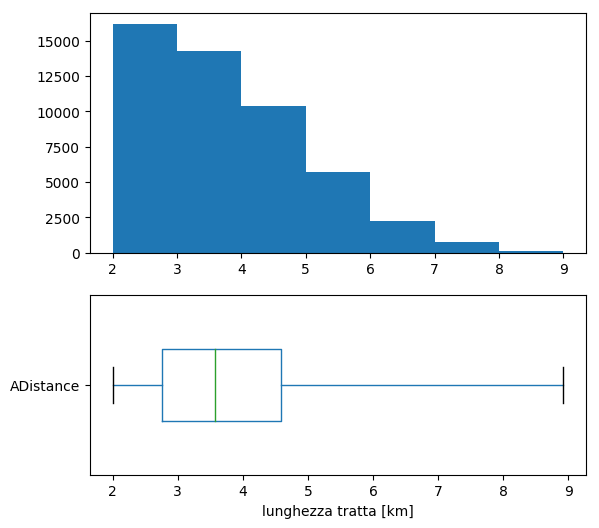
\includegraphics[scale=0.8]{distribuzione_tratte}
\caption{Frequenza assoluta lunghezza tratte [km]}
\label{image:2}
\end{figure}

\begin{figure}[H]
	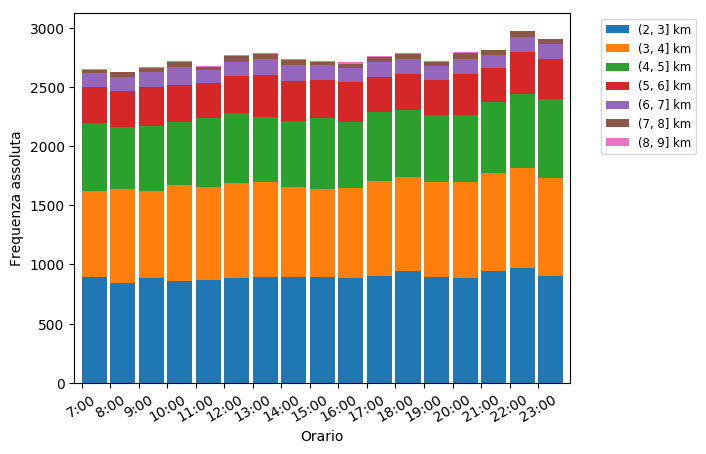
\includegraphics[scale=0.8]{distribuzione_tratte_oraria}
	\caption{Frequenza assoluta lunghezza tratte in base all'orario [km]}
	\label{image:19}
\end{figure}

\begin{table}[H]
\centering
\begin{tabular}{ | l r | }
\hline
\textbf{Abs. freq.} & 49560 \\
\textbf{Media} & 3.80 km \\
\textbf{Mediana} & 3.57 km \\
\textbf{Std} & 1.27 km \\
\textbf{Min} & 2.00 km \\
\textbf{Max} & 9.52 km \\
\hline
\end{tabular}
\caption{Statistiche lunghezza tratta [km]}
\label{table:2}
\end{table}

Nel grafico \ref{image:2} e nella tabella \ref{table:2} sono riportate le statistiche riguardo la lunghezza in via aerea delle tratte generate. Si può notare come più della metà siano lunghe meno di 5 km in linea aerea, risultato voluto e ottenuto dai constraint imposti nella generazione riguardanti l'area del Comune di Milano e per l'ingresso e l'uscita dal centro storico al semicentro. Il grafico \ref{image:19} mostra come la lunghezza delle tratte è stata equidistribuita nelle diverse fasce di orario.

\section{Performance dei singoli mezzi}

\begin{figure}[H]
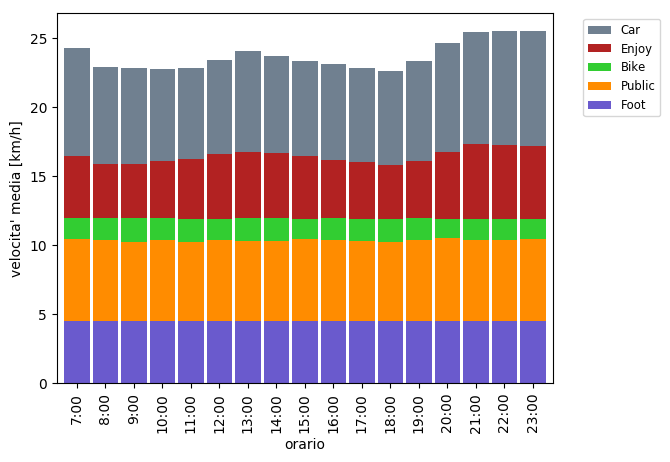
\includegraphics[scale=0.8]{vmedia_oraria_all}
\caption{Performance medie dei singoli mezzi per fascia oraria}
\label{image:15}
\end{figure}

\begin{table}[H]
\centering
\begin{tabular}{ | l r r r r r | }
\hline
& \textbf{Auto} & \textbf{Enjoy} & \textbf{Bici} & \textbf{ATM} & \textbf{Piedi} \\
\textbf{Media}      & 23.7 & 16.4 & 11.9 & 10.3 & 4.5 \\
\textbf{Mediana} & 23.6 & 16.2 & 11.9 &   9.8 & 4.5 \\
\textbf{Std}             &  3.9 &   4.2 &   1.3 &    3.0 & 0.0 \\
\textbf{Min}            &  8.9 &   3.5 &   6.5 &    3.7 & 4.3 \\
\textbf{Max}         & 59.0 & 46.4 & 16.9 &  41.0 & 4.6 \\
\hline
\end{tabular}
\caption{Statistiche velocità media [km/h]}
\label{table:3}
\end{table}

Dal grafico \ref{image:15} si può subito notare come i risultati dei tragitti a piedi, coi mezzi pubblici ATM e in bicicletta abbiano una bassa variazione in relazione all'orario, il che è un risultato aspettato visto che i servizi di navigazione per risolvere le richieste di viaggio non sono stati basati su dati in tempo reale ma statici, a differenza dei tragitti in auto e in Enjoy. Fatto confermato anche nella tabella \ref{table:3} dalla voce Std per deviazione standard. Si può notare inoltre come le velocità medie di percorrenza di mezzi pubblici e bicicletta siano molto vicini. Questi primi risultati sono in linea con quelli dell'ISFORT riportati nella tabella \ref{table:9}, che vede l'automobile in testa alla classifica intorno a 22 km/h di media, con la bici al secondo posto ma con 15 km/h e i mezzi pubblici al terzo con 14 km/h, stime poco più alte di quelle sopra riportate.

\subsection{Auto}

\subsubsection{Velocità media di ora in ora}

\begin{figure}[H]
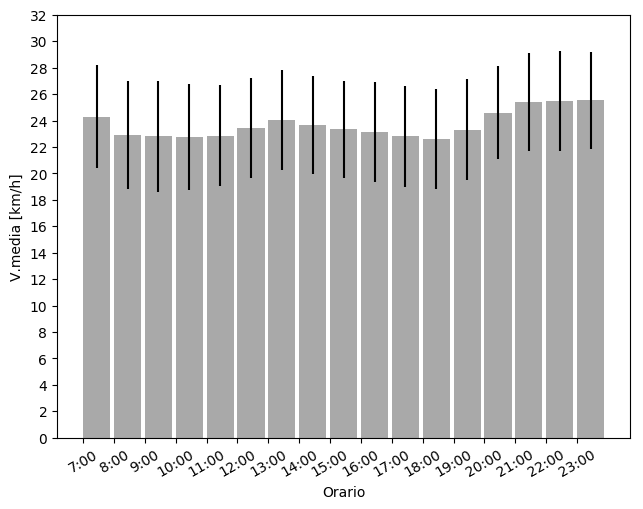
\includegraphics[scale=0.8]{vmedia_oraria_auto}
\caption{Velocità media in auto [km/h], di ora in ora}
\label{image:3}
\end{figure}

Una delle prime analisi effettuate per ogni mezzo è stata quella di calcolare la velocità media per ogni tragitto effettuato riguardante l'intero periodo di raccolta dati, con l'obbiettivo di osservare eventuali variazioni di ora in ora. Come riportato nel grafico \ref{image:3}, i tragitti in auto hanno subito una variazione di velocità media nell'arco 8:00-11:00 e in quello delle 17:00-19:00, in cui si registra la velocità media minima di 23 km/h. Tali risultati sono in linea, tra i tanti studi a riguardo del traffico in auto a Milano, con quelli dello studio di TomTom\cite{tomtomindexmilan} effettuato sulla città di Milano nel 2019, che evidenzia le ore 9:00 e 18:00, orari di picco del traffico stradale dal lunedì al venerdì, con un livello di congestione rispettivamente del 70\% e del 60\%. Risultano in linea con lo studio anche le ore precedenti e successive agli orari individuati come picchi. Si possono notale inoltre gli scarti quadratici medi evidenziati con i segmenti neri incastonati nelle barre, che risultano costanti a ogni orario. La massima velocità media si rileva nei tragitti dopo le 22:00, di circa 26 km/h.

\subsubsection{Velocità media lunedì-venerdì e sabato-domenica}

\begin{figure}[H]
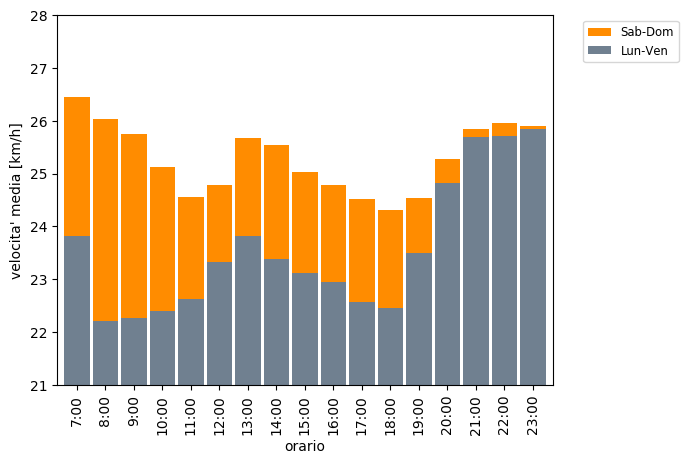
\includegraphics[scale=0.8]{vmedia_oraria_auto_weekend}
\caption{Velocità media in auto [km/h], di ora in ora}
\label{image:4}
\end{figure}

\begin{table}[H]
\centering
\begin{tabular}{ | l r r r r r r r r r | }
\hline
\textbf{Orario} & \textbf{7:00} & \textbf{8:00} & \textbf{9:00} & \textbf{10:00} & \textbf{11:00} & \textbf{12:00} & \textbf{13:00} & \textbf{14:00} & \textbf{15:00} \\
\textbf{Km/h}& 2.6 & 3.8 & 3.4 & 2.7 & 1.9 & 1.4 & 1.8 & 2.1 & 1.9 \\
\textbf{\%}    & 9.9 & 14.6  & 13.5 & 10.8 & 7.8 & 5.8 & 7.2 & 8.4 & 7.6 \\
\hline
\textbf{Orario} & \textbf{16:00} & \textbf{17:00} & \textbf{18:00} & \textbf{19:00} & \textbf{20:00} & \textbf{21:00} & \textbf{22:00} & \textbf{23:00} & \quad \\
\textbf{Km/h}&  1.8 & 1.9 & 1.8 & 1.0 & 0.4 & 0.1 & 0.2 & 0.0 & \quad \\
\textbf{\%}    & 7.4 & 7.9 & 7.6 & 4.2 & 1.8 & 0.6 & 0.9 & 0.2 & \quad \\
\hline
\end{tabular}
\caption{Differenza velocità media tra week e weekend [km/h]}
\label{table:8}
\end{table}

Il grafico \ref{image:4} mostra il risultato di una ripartizione dei dati effettuata sulla base del giorno della settimana, in particolare sono stati divisi i tragitti effettuati dal lunedì al venerdì da quelli del sabato e domenica di ogni settimana. La differenza è nel complesso bassa, di circa 2 km/h di media, che tende a diminuire negli orari notturni. La massima differenza di velocità media si ottiene nei tragitti nella fascia oraria delle ore 8, con una differenza di quasi 4 km/h che corrisponde a un incremento della velocità media del 14.6\% in più rispetto al lunedì-venerdì, come riportato dalla tabella \ref{table:8}. La variazione nel sabato-domenica risulta meno evidente di quella del lunedì-venerdì, con le variazioni, ovvero i picchi di rallentamento, che si spostanto nelle fasce orarie 10:00-12:00 e 16:00-19:00. Anche questi dati risultano in linea con quelli dello studio di TomTom\cite{tomtomindexmilan}, che vede un minor livello di congestione nel weekend con dei picchi nelle ore 10:00 e 18:00. La deviazione standard delle fasce di orario del lunedì-venerdì rimangono invariate anche nel sabato-domenica, seppur non riportate per motivi di leggibilità.

\subsubsection{Velocità media settimana dopo settimana da fine lockdown}

\begin{figure}[H]
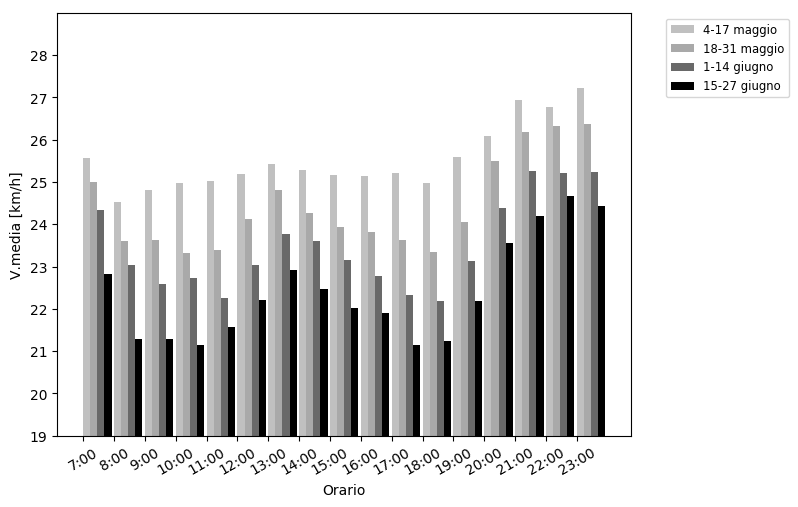
\includegraphics[scale=0.8]{vmedia_oraria_auto_weeks}
\caption{Velocità media in auto [km/h], di ora in ora}
\label{image:5}
\end{figure}

Il grafico \ref{image:5} mostra il risultato di una ripartizione dei dati effettuata in base alla settimana, in particolare sono stati partizionati a gruppi di 2 settimane consecutive i tragitti effettuati a partire dal 4 maggio 2020, primo giorno dell'allentamento delle restrizioni imposte dal governo italiano per l'emergenza COVID-19\cite{dpcm26aprile}. Nel grafico risulta evidente una degradazione della velocità media generale e lineare rispetto al passare delle settimane. Si nota inoltre che le curve corrispondenti alle settimane successive al 17 maggio, ovvero dopo le prime 2 settimane, presentino dei flessi sempre più accentuati in prossimità degli orari di picco del traffico evidenziati dal grafico \ref{image:3}. Anche in questo caso, non sono state riportate differenze nella deviazione standard.

\subsubsection{Velocità media in base alla lunghezza tratta}

\begin{figure}[H]
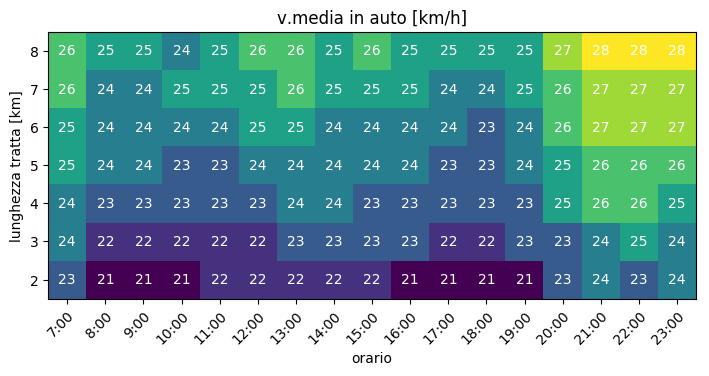
\includegraphics[scale=0.75]{heatmap_auto}
\caption{Velocità media in auto [km/h] in base alla lunghezza tratta, di ora in ora}
\label{image:6}
\end{figure}

Nel grafico \ref{image:6} sono riportati i dati della velocità media divisi per fasce d'orario e lunghezza in chilometri della tratta tramite una heatmap. Si evidenziano due gobbe in corrispondenza degli orari di picco del traffico intorno alle ore 9:00 e 18:00, e le tratte brevi lunghe dai 2 ai 3 chilometri risultano le più colpite. Si evidenzia inoltre un'altra area di forma rettangolare di colori chiari a partire dalle ore 20:00, dove la velocità media si stabilizza per tutte le fasce di lunghezza intorno ai 27 km/h.

\subsection{Enjoy}

\subsubsection{Velocità media di ora in ora}

\begin{figure}[H]
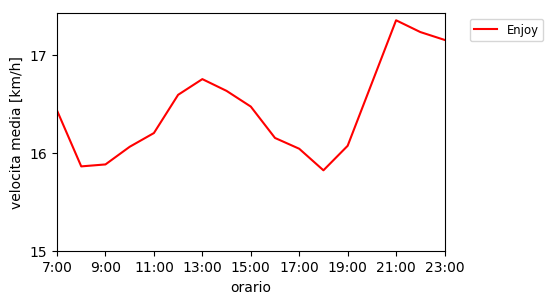
\includegraphics[scale=0.8]{vmedia_oraria_enjoy}
\caption{Velocità media usando Enjoy [km/h], di ora in ora}
\label{image:7}
\end{figure}

I tragitti col servizio di car sharing Enjoy hanno subito una lieve variazione di velocità media nell'arco 8:00-11:00 e in quello delle 17:00-19:00 come per l'auto di proprietà, in cui si registra la velocità media minima di 16 km/h, seppur la massima registrata sia stata di 17 km/h. La variazione è all'atto pratico poco significativa. La deviazione standard rimane costante per tutte le fasce di orario. Rispetto al grafico \ref{image:3} della velocità media in auto, la curva risulta molto simile, traslata verticalmente di 6 km/h.

\subsubsection{Velocità media lunedì-venerdì e sabato-domenica}

\begin{figure}[H]
	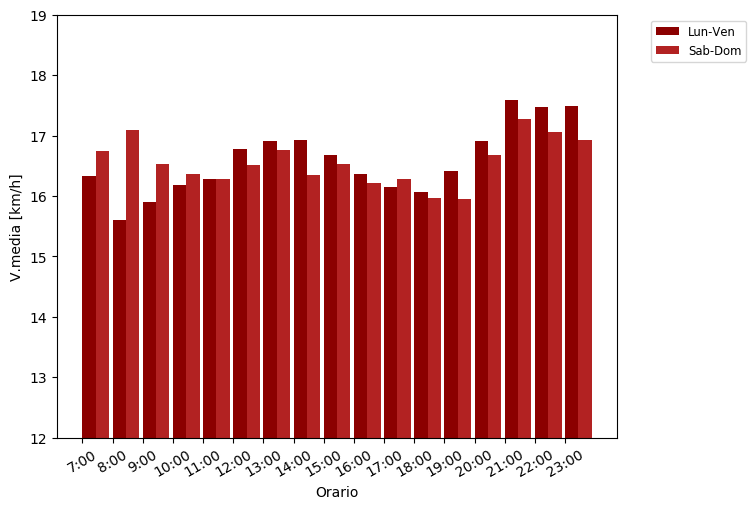
\includegraphics[scale=0.8]{vmedia_oraria_enjoy_weekend}
	\caption{Velocità media usando Enjoy [km/h], di ora in ora}
	\label{image:20}
\end{figure}

Non sono state registrate particolari differenze effettuando la ripartizione dei dati in base al giorno della settimana, come mostrato nella figura \ref{image:20}. La velocità media rimane costante, con una lieve differenza nella fascia oraria delle 8:00. La deviazione standard, rimane costante e identica a quella del grafico \ref{image:7}.

\subsubsection{Velocità media settimana dopo settimana da fine lockdown}

\begin{figure}[H]
	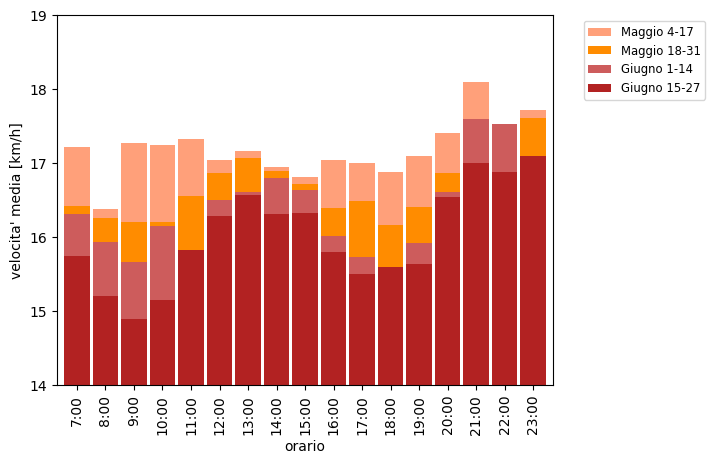
\includegraphics[scale=0.8]{vmedia_oraria_enjoy_weeks}
	\caption{Frequenza relativa vittorie bicicletta su Enjoy di ora in ora}
	\label{image:16}
\end{figure}

Anche per il car sharing Enjoy, nel grafico \ref{image:16} risulta evidente una degradazione della velocità media generale e lineare rispetto al passare delle settimane. Non risultano differenze nelle fasce orarie meno trafficate dalle 12:00 alle 15:00 e dalle 21:00 alle 23:00. Le prime due settimane dall'allentamento delle restrizioni risultano più veloci di circa 1 km/h di media dalle altre settimane.

\subsubsection{Auto libere e tempo medio per raggiungerle}

\begin{table}[H]
\centering
\begin{tabular}{ | l r | }
\hline
& \textbf{T.medio ragg.auto} \\
\textbf{Media}   &  6.6 \\
\textbf{Mediana} &  6.0 \\
\textbf{Std}     &  4.6 \\
\textbf{Min}     &  0.0 \\ 
\textbf{Max}     & 43.0 \\
\hline
\end{tabular}
\caption{Statistiche tempo medio per raggiungere auto libera [min]}
\label{table:4}
\end{table}

\begin{figure}[H]
	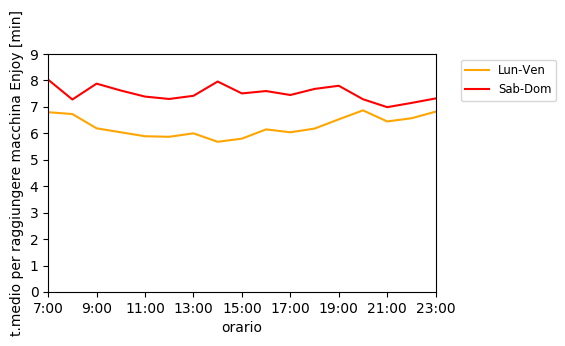
\includegraphics[scale=0.8]{tmedio_raggiungimento_auto_enjoy}
	\caption{Tempo medio per raggiungere auto libera [min], di ora in ora}
	\label{image:8}
\end{figure}

Sottraendo il tempo impiegato in auto da quello impiegato col car sharing Enjoy è stata ottenuta una stima indicativa del tempo medio per raggiungere un'auto libera a piedi. Dai calcoli è risultato che il tempo medio oscilla intorno ai 6 minuti e mezzo, come riportato dalla tabella \ref{table:4}. Anche per questa analisi i dati sono stati partizionati per i giorni da lunedì a venerdì e per sabato e domenica. Il box plot della figura \ref{image:8} evidenzia il range interquantile nell'intervallo dai 3 ai 9 minuti, con una mediana di 6. Il tempo medio per raggiungere un'auto Enjoy, di 6.6 minuti, sembra coincidere con la differenza di velocità media rispetto ai dati dell'auto privata, citata sotto il grafico \ref{image:7}.

\begin{figure}[H]
	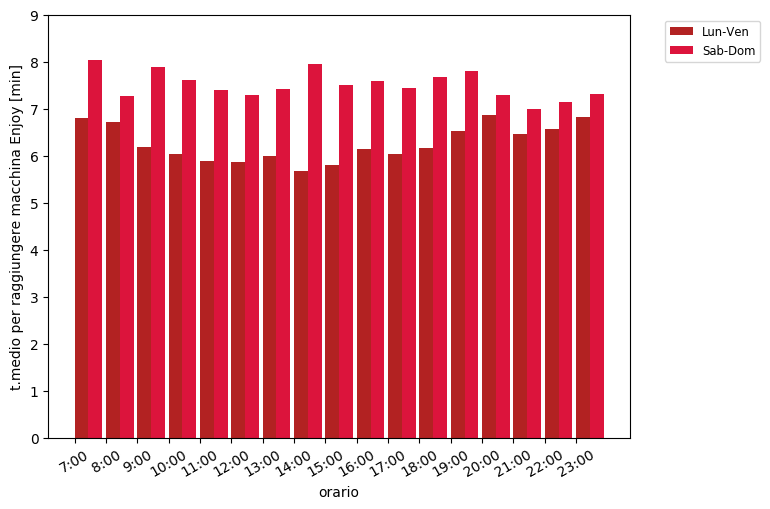
\includegraphics[scale=0.8]{tmedio_raggiungimento_auto_enjoy_weekend}
	\caption{Tempo medio per raggiungere auto libera [min]}
	\label{image:21}
\end{figure}

Il grafico \ref{image:8} mostra una lieve differenza nel tempo medio per raggiungere un'auto libera Enjoy di circa 1 minuto a sfavore dei giorni del fine settimana. Dunque, in settimana le auto risultano più vicine o più facilmente raggiungibili.

\begin{figure}[H]
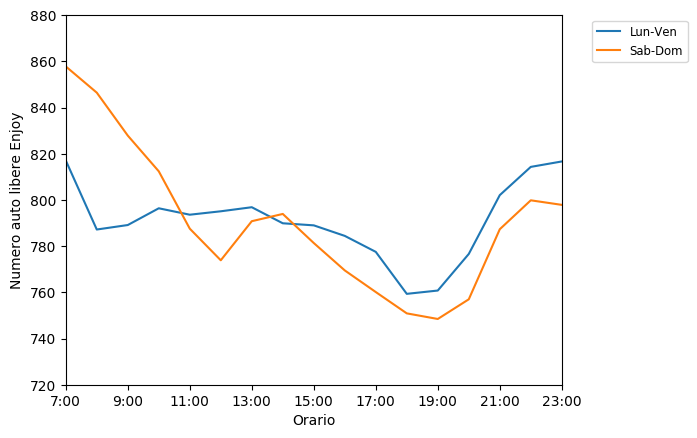
\includegraphics[scale=0.8]{variazione_auto_libere_enjoy_weekend}
\caption{Numero di auto libere Enjoy lungo l'arco della giornata}
\label{image:9}
\end{figure}

Per contestualizzare il tempo medio per raggiungere un'auto Enjoy è stato usato il dato sul numero delle macchine libere salvato per ogni query ai servizi. Il massimo numero di auto libere in circolazione è stato di 870. Nel grafico \ref{image:9} viene mostrata in media la variazione di questo conteggio lungo l'arco della giornata, ripartito per lunedì-venerdì e sabato-domenica. Si può notare come il picco di utilizzo del servizio, denotato da un calo delle auto libere a disposizione, inizia verso le 15:00 e finisce verso le 21:00 indipendentemente dal giorno. L'unica differenza tra i due gruppi si può notare nelle ore del mattino, che vede meno auto libere durante la settimana.

Come è stato fatto con la velocità media per l'auto di proprietà, è stato calcolato il tempo medio per raggiungere un'auto libera Enjoy di settimana in settimana dalla fine del lockdown. Il risultato ottenuto è stato controintuitivo, mostrando come, col passare del tempo, il tempo medio per raggiungere un'auto libera diminuiva. Risulta controintuitivo infatti se si pensa al risultato ottenuto con la velocità media in auto, che ha visto una degradazione delle performance col ritorno alla normalità per quanto riguarda la mobilità. Analogamente si è pensato che il numero di utenti del servizio car sharing sarebbe aumentato col ritorno alla normalità e che quindi il tempo medio per raggiungere un auto sarebbe aumentato col diminuire delle auto libere in circolazione. Per investigare a fondo questo risultato è stato calcolato il numero di auto libere di settimana in settimana.

\begin{figure}[H]
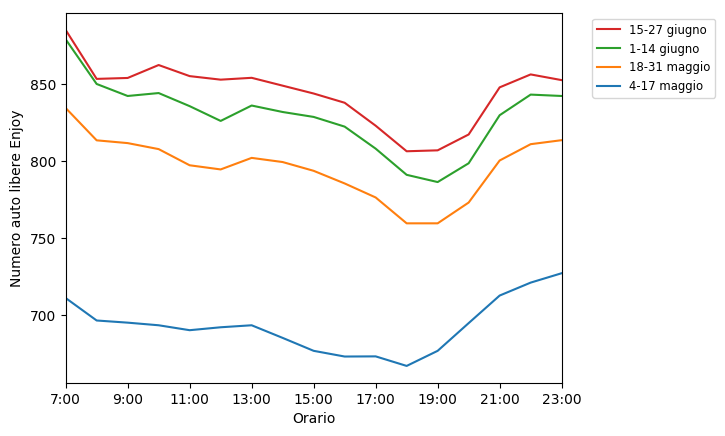
\includegraphics[scale=0.8]{variazione_auto_libere_enjoy_weeks}
\caption{Numero di auto libere Enjoy lungo settimana dopo settimana}
\label{image:10}
\end{figure}

Il grafico \ref{image:10} mostra chiaramente come il numero delle auto libere a disposizione sia aumentato con la fine del lockdown. Si può notare infatti come siano state immesse circa 150 nuove auto nell'arco di un mese e altre 50 nel mese successivo. Questo dato di fatto sembra risolvere il risultato controintuitivo ottenuto nell'analisi precedente.


\subsection{Mezzi pubblici ATM, bici e a piedi}

\subsubsection{Velocità media di ora in ora}

\begin{figure}[H]
	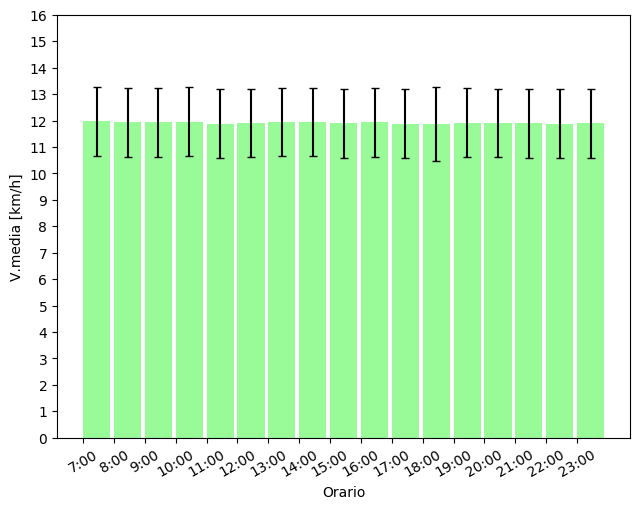
\includegraphics[scale=0.8]{vmedia_oraria_bici}
	\caption{Frequenza relativa vittorie bicicletta su Enjoy di ora in ora}
	\label{image:11}
\end{figure}

\begin{figure}[H]
	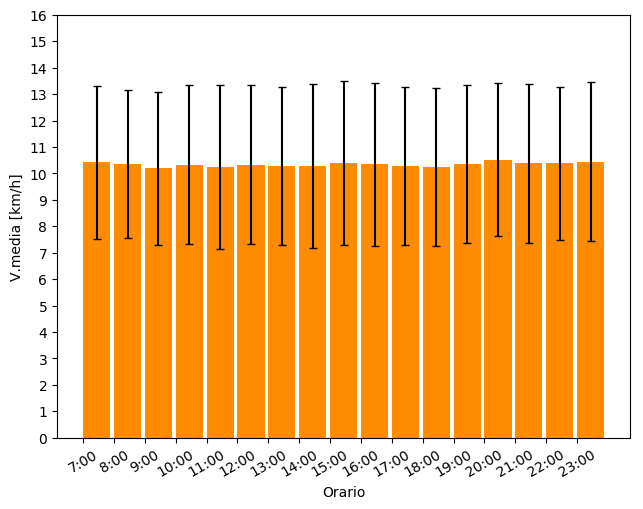
\includegraphics[scale=0.8]{vmedia_oraria_atm}
	\caption{Frequenza relativa vittorie bicicletta su Enjoy di ora in ora}
	\label{image:17}
\end{figure}

\begin{figure}[H]
	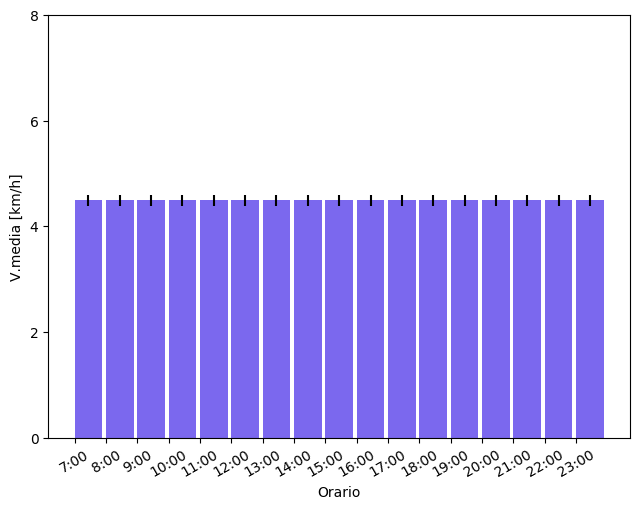
\includegraphics[scale=0.8]{vmedia_oraria_piedi}
	\caption{Frequenza relativa vittorie bicicletta su Enjoy di ora in ora}
	\label{image:18}
\end{figure}

Analizzando le stime di percorrenza riguardo i mezzi pubblici, la bicicletta e i percorsi a piedi, non si è verificata alcuna variazione significativa lungo l'arco della giornata, tradotto graficamente come nei grafici \ref{image:11}, \ref{image:17} e \ref{image:18} in una retta parallela all'asse x per ognuno dei mezzi considerati. Il risultato è aspettato, dato che tali servizi non hann fornito risposte dinamiche in base alle condizioni attuali del traffico e dei dati storici, e, nel caso della bicicletta e a piedi, perchè l'influenza è praticamente nulla per questi mezzi di trasporto.

\section{Confronto tra mezzi}

In questo paragrafo sono stati raccolti i risultati più interessanti emersi dal confronto tra tutti i mezzi di trasporto a disposizione per spostarsi nel Comune di Milano. Il confronto più atteso che ha fatto da guida verso questo studio è stato quello di verificare se un mezzo altamente costoso e inquinante come le auto a gasolio e benzina potessero essere surclassate da un mezzo più economico e pulito come i mezzi pubblici in una città dove il traffico influisce pesantemente sui tempi di percorrenza, come mostrato nel grafico \ref{image:3}.

\subsection{Vittoria dell'automobile}

Contro ogni aspettativa, nonostante la grande influenza del traffico sui tempi di percorrenza, i tragitti in auto sono risultati sempre i più veloci di ogni sua controparte, a qualsiasi ora del giorno e su ogni distanza, con una vittoria sopra il 99\% delle volte.

\subsection{Parziale sconfitta del car sharing}

\subsubsection{Mezzi pubblici ATM vs. Enjoy}

\begin{table}[H]
\centering
\begin{tabular}{ | r r r | }
\hline
& \textbf{Abs. freq.} & \textbf{\% win} \\
\textbf{(2, 5] km} & 2072 & 4.2 \\
\textbf{(5, 7] km} & 1512 & 3.1 \\
\textbf{(7, 10] km} & 670 & 1.4 \\
\hline
\textbf{totale} & 4294 & 8.7 \\
\hline
\end{tabular}
\caption{Vittoria dei mezzi pubblici su car sharing per lunghezza tratta}
\label{table:5}
\end{table}

\begin{figure}[H]
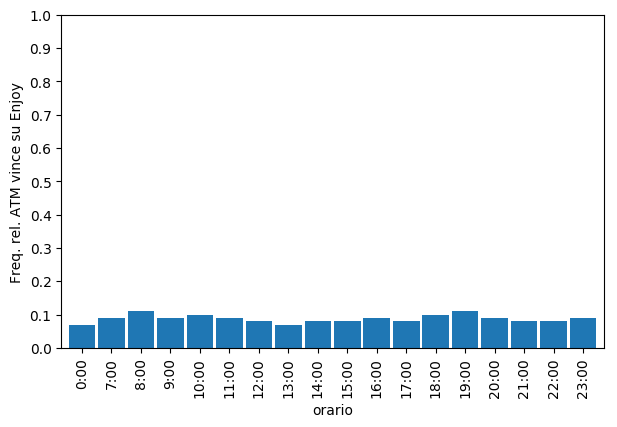
\includegraphics[scale=0.8]{confronto_atm_enjoy}
\caption{Frequenza relativa vittorie ATM su Enjoy di ora in ora}
\label{image:13}
\end{figure}

I risultati del confronto tra i mezzi pubblici ATM e il servizio di car sharing Enjoy illustrati nella tabella \ref{table:5} mostrano una percentuale di vittorie di circa il 9\%, dove per vittoria si intende che il tempo impiegato a percorrere una tratta coi mezzi pubblici è stato minore o uguale al tempo impiegato utilizzando il car sharing. Nel grafico \ref{image:13} viene visualizzata la distribuzione di queste vittorie di ora in ora. Si può notare come vicino alle ore di picco del traffico individuate nell'analisi delle performance dell'auto, ovvero le ore 8:00-10:00 e 17:00-20:00, si concentri la percentuale maggiore di sconfitte da parte del car sharing.

Per esempio, su tutte le tratte richieste nelle ore 8:00, nell'11\% delle volte i mezzi pubblici hanno pareggiato o superato la performance del car sharing. Al contrario, al di fuori degli orari di picco del traffico, la percentuale di vittorie è vicina allo 0. Dalla tabella \ref{table:5} si evince anche che dell'8.7\% di queste vittorie, circa metà di esse sono tratte brevi dai 2 ai 5 km.

\subsubsection{Bicicletta vs. Enjoy}

\begin{table}[H]
\centering
\begin{tabular}{ | r r r | }
\hline
& \textbf{Abs. freq.} & \textbf{\% win} \\
\textbf{(2, 5] km} & 15215 & 30.7 \\
\textbf{(5, 7] km} & 2423 & 4.9 \\
\textbf{(7, 10] km} & 278 & 0.6 \\
\hline
\textbf{totale} & 17917 & 36.2 \\
\hline
\end{tabular}
\caption{Vittoria della bicicletta su car sharing per lunghezza tratta}
\label{table:6}
\end{table}

\begin{figure}[H]
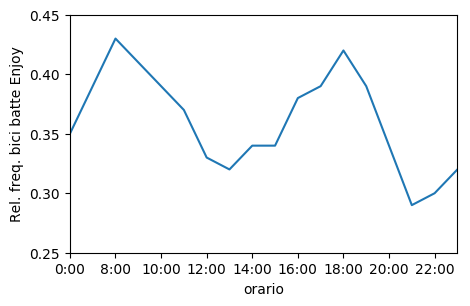
\includegraphics[scale=0.8]{confronto_bike_enjoy}
\caption{Frequenza relativa vittorie bicicletta su Enjoy di ora in ora}
\label{image:14}
\end{figure}

Risultato ancora più interessante è quello del confronto tra bicicletta di proprietà e car sharing. La tabella \ref{table:6} mostra una percentuale delle vittorie del 36\% sul totale, poco più di un terzo del totale delle tratte. La maggior parte di queste vittorie è concentrata nelle tratte brevi dai 2 ai 5 km.

Anche in questo confronto è emerso che negli orari di picco si accentua la percentuale di vittorie che arriva a toccare quasi il 45\% del totale nelle ore 8:00 e 18:00 come riportato dal grafico \ref{image:14}. Al contrario dei mezzi pubblici, questa percentuale resta alta anche al di fuori degli orari di punta, restando sempre intorno al 30\%.

\section{Confronto pre e post lockdown}

Nonostante le prime versioni del programma di raccolta dati abbiano portati a diversi dati nulli, le stime relative al percorso in automobile e in car sharing sono sempre state corrette. Si è deciso quindi di analizzare l'unica settimana a disposizione prima del lockdown, dal lunedì 2 marzo a domenica 8 marzo 2020, rappresentativa di una giornata tipo a livello di traffico stradale, con una delle settimane più trafficate dopo il lockdown, che dalle analisi riportate dalla figura \ref{image:5} e \ref{image:16} sono risultate corrispondenti al periodo dal 15 giugno al 27 giugno 2020.

\subsection{Automobile}

\begin{figure}[H]
	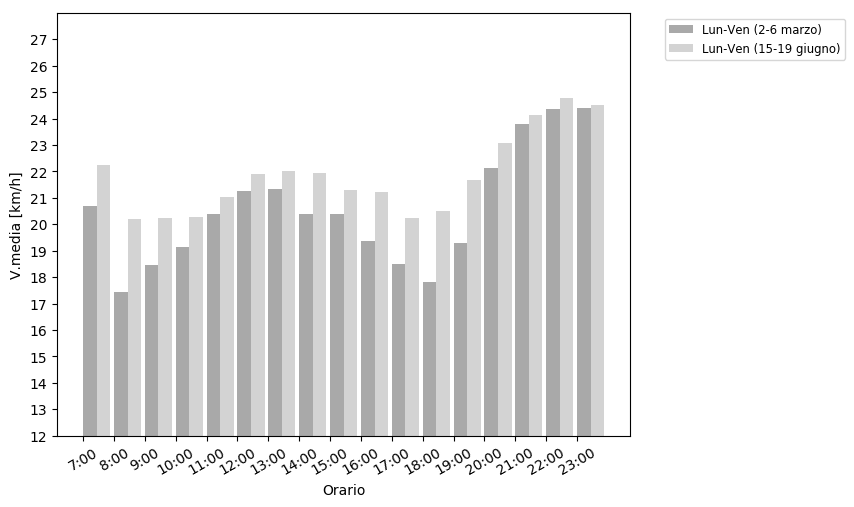
\includegraphics[scale=0.8]{vmedia_oraria_auto_prepostlock_week}
	\caption{V.media [km/h] auto di ora in ora pre e post lockdown}
	\label{image:22}
\end{figure}

\begin{figure}[H]
	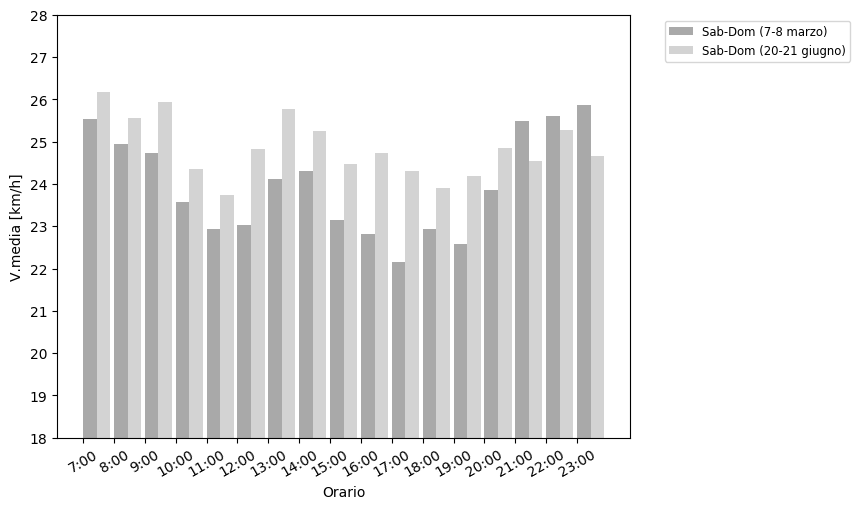
\includegraphics[scale=0.8]{vmedia_oraria_auto_prepostlock_weekend}
	\caption{V.media [km/h] auto di ora in ora pre e post lockdown}
	\label{image:23}
\end{figure}

Nel grafico \ref{image:22} si può notare una lieve differenza di km/h di media tra una settimana pre e post lockdown intrasettimanale. Questa differenza risulta più evidente negli orari di picco del traffico vicino alle 8:00 e alle 18:00, con una differenza di 2 km/h di media. Risulta evidente inoltre la differenza di velocità media nel pre lockdown tra le 8:00, dove si tocca il minimo di 17.5 km/h, alle 23:00, dove si trova il massimo di 24.5 km/h, una differenza di velocità del 28\%. Risulta meno evidente ma pur sempre presente la differenza nel weekend come mostrato dal grafico \ref{image:23}, che vede la più grande differenza nel pomeriggio intorno alle 16:00, di circa 2 km/h.

\subsection{Enjoy}

\begin{figure}[H]
	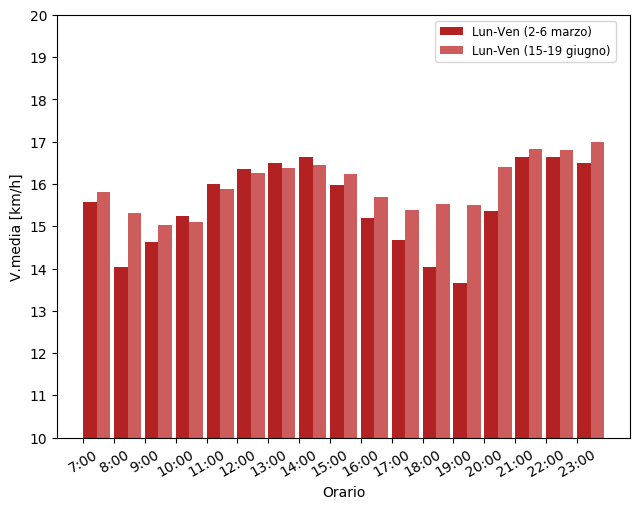
\includegraphics[scale=0.8]{vmedia_oraria_enjoy_prepostlock_week}
	\caption{V.media [km/h] Enjoy di ora in ora pre e post lockdown}
	\label{image:24}
\end{figure}

\begin{figure}[H]
	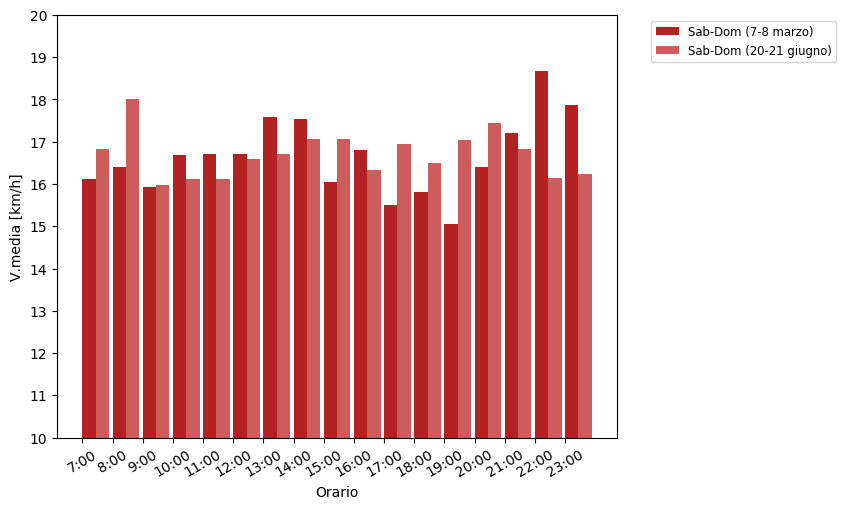
\includegraphics[scale=0.8]{vmedia_oraria_enjoy_prepostlock_weekend}
	\caption{V.media [km/h] Enjoy di ora in ora pre e post lockdown}
	\label{image:25}
\end{figure}

I tempi di percorrenza in car sharing Enjoy sono risultati molto simili, come mostrato dal grafico \ref{image:24}. La maggior differenza è presente anche questa volta vicino le ore di picco delle 8:00 e delle 18:00, sebbene la differenza sia minima, di media 1 km/h. Lo stesso discorso si può fare anche nel weekend, come mostrato nel grafico \ref{image:25}. Una sostanziale differenza si può notare inoltre nell'orario notturno delle 22:00 e delle 23:00, che vede nel periodo post lockdown una minore velocità media di circa 2 km/h.













